\subsection{Energiekalibration}
Für beide Detektoren wird ein Zusammenhang zwischen den Bins des MCA und der dem Signal entsprechenden Energie hergestellt. Dazu wird zunächst an die aufgenommenen \SI{511}{\kilo\electronvolt} Linien eine Gaußfunktion
\begin{align}
  N(n)=A \exp \left( -\frac{(n-\mu)}{2 \sigma^2} \right)
  \label{eq:gauss}
\end{align}
mit Gnuplot angepasst. Die resultierenden Parameter sind
\begin{align*}
  A_l&=195,4 \pm 0,9\\
  \mu_l&=7469,1 \pm 0,9\\
  \sigma_l&=261,1 \pm 0,8\\
  A_r&=168 \pm 1\\
  \mu_r&=6669 \pm 1\\
  \sigma_r&=227 \pm 1
\end{align*}
Die Spektren mit den angepassten Regressionskurven sind in Abbildung \ref{fig:511} zu sehen.
\begin{figure}[h]
  \centering
  \begin{subfigure}[h]{0.5\textwidth}
    \centering
    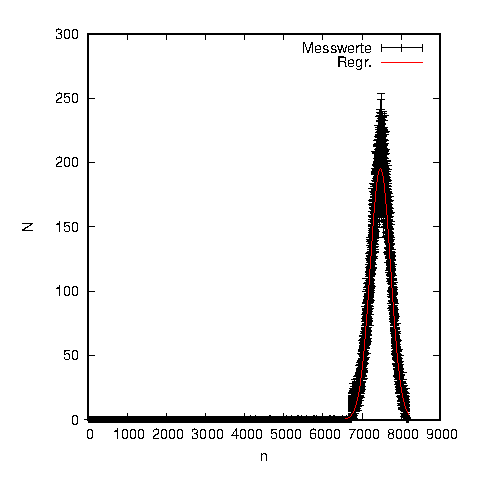
\includegraphics[width=0.9\textwidth]{data/Energiespektren/na_kal_links.eps}
    \subcaption{linker Detektor}
    \label{fig:511_links}
  \end{subfigure}%
  \begin{subfigure}[h]{0.5\textwidth}
    \centering
    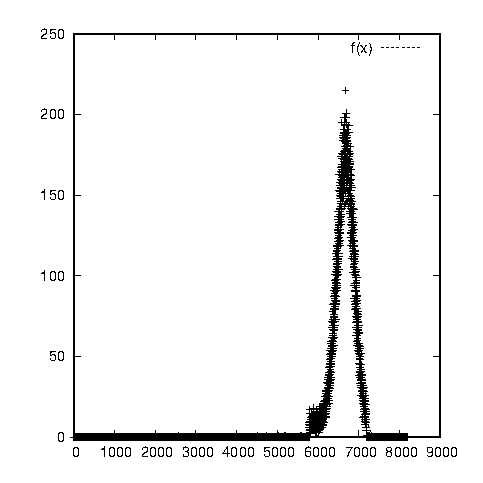
\includegraphics[width=0.9\textwidth]{data/Energiespektren/na_kal_rechts.eps}
    \subcaption{rechter Detektor}
    \label{fig:511_rechts}
  \end{subfigure}
  \caption{mit beiden Detektoren aufgenommene \SI{511}{\kilo\electronvolt} Linien}
  \label{fig:511}
\end{figure}

In den aufgenommenen Spektren von $^{133}$Ba sind sieben Peaks zu erkennen. An die Spektren wird eine Superposition von sieben Gaußkurven (siehe Gleichung (\ref{eq:gauss})) und einer Gerade $a\cdot n+b$ angepasst. Die Spektren mit den angepassten Funktionen sind in Abbildung \ref{fig:ba_kal} zu sehen. Die Parameter der Regressionskurven befinden sich im Anhang in Tabelle \ref{tab:ba_rechts} und \ref{tab:ba_links}. \newpage
\begin{figure}[h]
  \centering
  \begin{subfigure}[h]{0.5\textwidth}
    \centering
    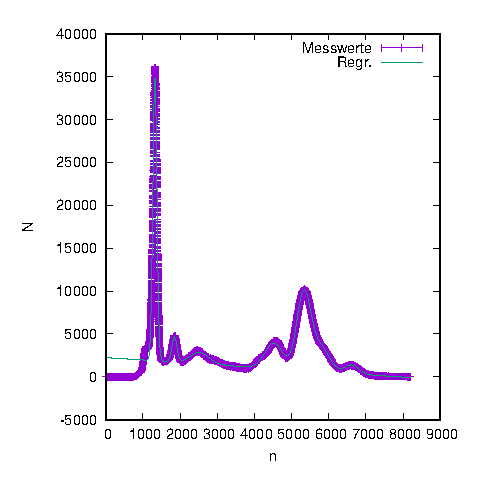
\includegraphics[width=0.9\textwidth]{data/Energiespektren/links_ba_cfd_kal.eps}
    \subcaption{linker Detektor}
    \label{fig:ba_kal_links}
  \end{subfigure}%
  \begin{subfigure}[h]{0.5\textwidth}
    \centering
    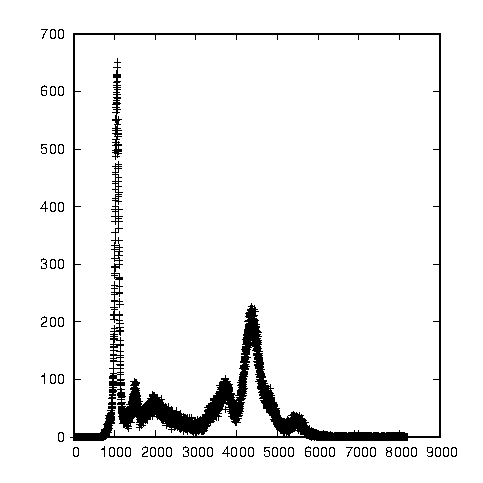
\includegraphics[width=0.9\textwidth]{data/Energiespektren/rechts_ba_cfd_kal.eps}
    \subcaption{rechter Detektor}
    \label{fig:ba_kal_rechts}
  \end{subfigure}
  \caption{mit beiden Detektoren aufgenommenes Spektrum von $^{133}$Ba}
  \label{fig:ba_kal}
\end{figure}
